\documentclass[10pt]{article}
\usepackage[letterpaper,margin=0.7in]{geometry}
\usepackage{graphicx}
\usepackage{amsmath}
\usepackage[T1]{fontenc}
\usepackage{hyperref}
\hypersetup{pdftitle={FROB C5 characteristic-five countercontrol},
  pdfsubject={EXP-FROB-91ee9c C5; repeated factor at characteristic five}}
\setlength{\parindent}{0pt}
\setlength{\parskip}{0.5em}
\title{FROB C5 characteristic-five countercontrol}
\author{Validation audit, 22 October 2026}
\date{}
\begin{document}
\maketitle
\vspace{-2em}

\textbf{Question.} What happens to the coprime-factor kernel argument used
for the archived $q=11,13,19$ cells if the characteristic equals the
Frobenius order five? This is a mathematical negative control, not a new run.

\textbf{Lean result.} Over $\mathbf F_5$ the source proves
\[
X^5-1=(X-1)^5,\qquad
X^4+X^3+X^2+X+1=(X-1)^4.
\]
Consequently $X^5-1$ is not squarefree: the nonunit $X-1$ has a square
dividing it. The exact target theorem is
\texttt{CharacteristicFive.x\_pow\_five\_sub\_one\_not\_squarefree}.

\textbf{Proof method.} Mathlib's characteristic-five binomial identity
establishes the fifth-power equation. Ring normalization and checked
$\mathbf F_5$ coefficient identities establish the degree-four equation.
The squarefreeness definition then contradicts the degree-one, nonunit
divisor $X-1$. The Lean source commit begins
\texttt{203cff284eff}; the attached
verifier receipt binds that source and pinned Lean 4.35.0-rc1. The 8,971-job
workspace and 3,092-job target builds passed; 588 theorem declarations used
standard axioms only, and the target axiom audit passed. Independent semantic
review remains pending.

\textbf{Interpretation.} The coprime-factor CRT premise fails at
characteristic five. This does not contradict the q=11/13/19 mathematical
identities in companion PR \#2475. The archived trial contains no q=5 core
cell. Its quotient-field implementation, historical C5/C8 verdicts, source
custody and performance claims are not certified by this theorem.

\textbf{Graphs.} The diagram on page two is a boundary map. No numerical
performance graph or dashboard row changes because no measurement was made.

\newpage
\begin{center}
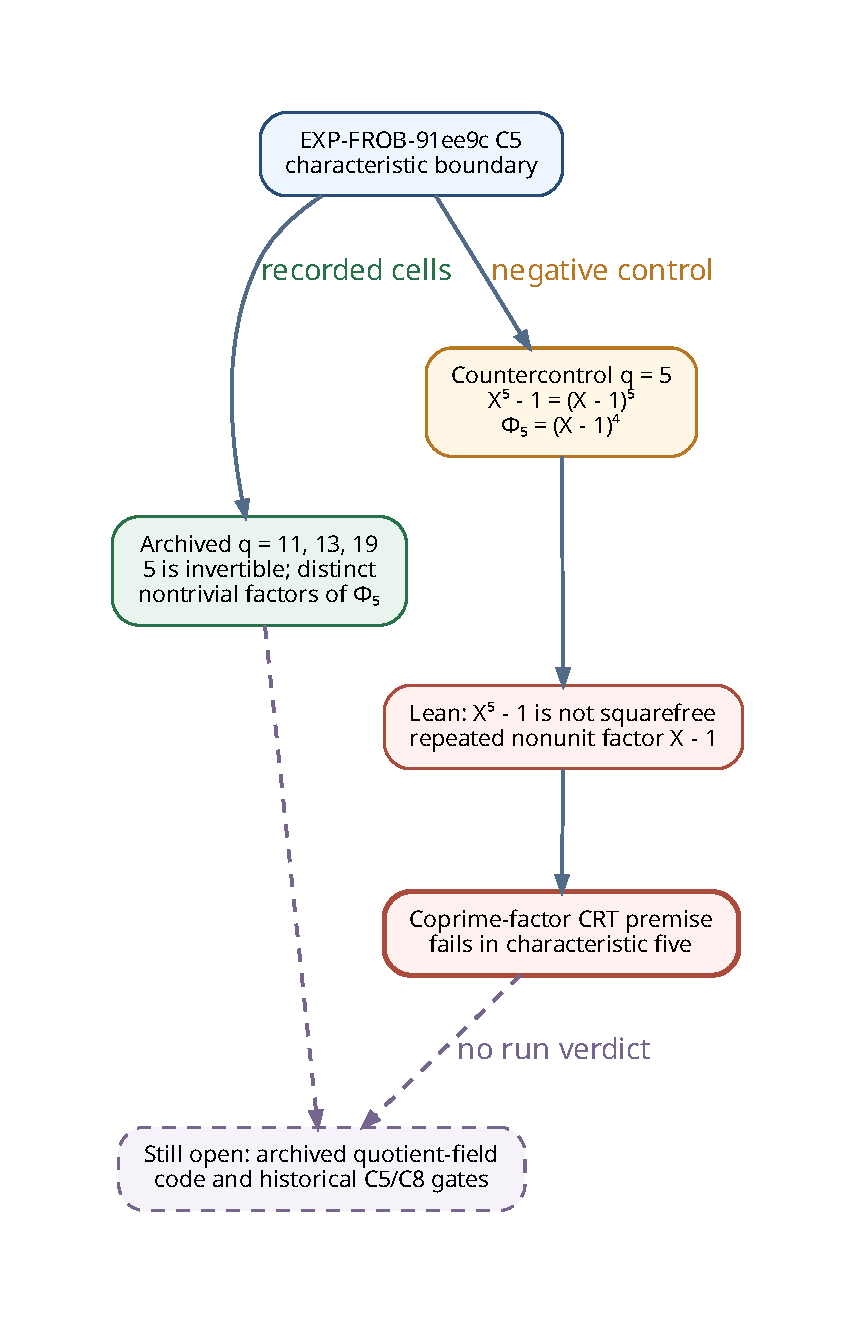
\includegraphics[width=\textwidth,height=0.88\textheight,keepaspectratio]{proof-figure.pdf}
\end{center}
\end{document}
